%--------------------------------------------------------------------------
% !TEX root = 5Blman.tex
% reflect.tex
% 2013.01.08 changed to 2col format
%--------------------------------------------------------------------------
\chapter{Reflection and Refraction}

\begin{multicols}{2}
%---------------------------------------------------------------------
\section{Purpose}
  The purpose of these laboratory exercises is to give you hands-on experience with the two basic laws of geometrical optics the laws of reflection and refraction. This lab continues the study of light, in particular the ray nature of light when light interacts with objects that are much larger than its wavelength.
  
%---------------------------------------------------------------------
\section{Preparation}
Note the definitions of important concepts in your text.  Pay particular attention to the laws of reflection and refraction.  Be certain you are comfortable with the ray model of light and the manner in which angles are denoted to specify the direction of a light ray.
\paragraph{Short quiz}
  Be prepared to take a short quiz at the beginning of lab related to the concepts associated with this laboratory exercise.
\section{General Information}

\paragraph{Warning}
  Never look directly into a laser beam and do not shine the beam into anyone's eye.  The lasers used in this laboratory are considered to be relatively safe, but should be treated with caution since lasers that are similar in appearance can have intensities great enough to do permanent harm to the eye.  
  
We use lasers in this laboratory exercise because they produce a narrow beam of monochromatic light.  The path of the light can therefore be more accurately determined than with other light sources.  (This underlies many of the applications of lasers.)  The path of light is a straight line until it interacts with some object.  When light encounters an object that is much larger than its wavelength  (as is the case in this laboratory exercise), it behaves like a ray and its direction is changed in accordance with the laws of reflection and refraction.
 
To measure the direction of a ray of light produced by a laser we use the set up shown here schematically.

%\begin{figure}
%	\centering
%	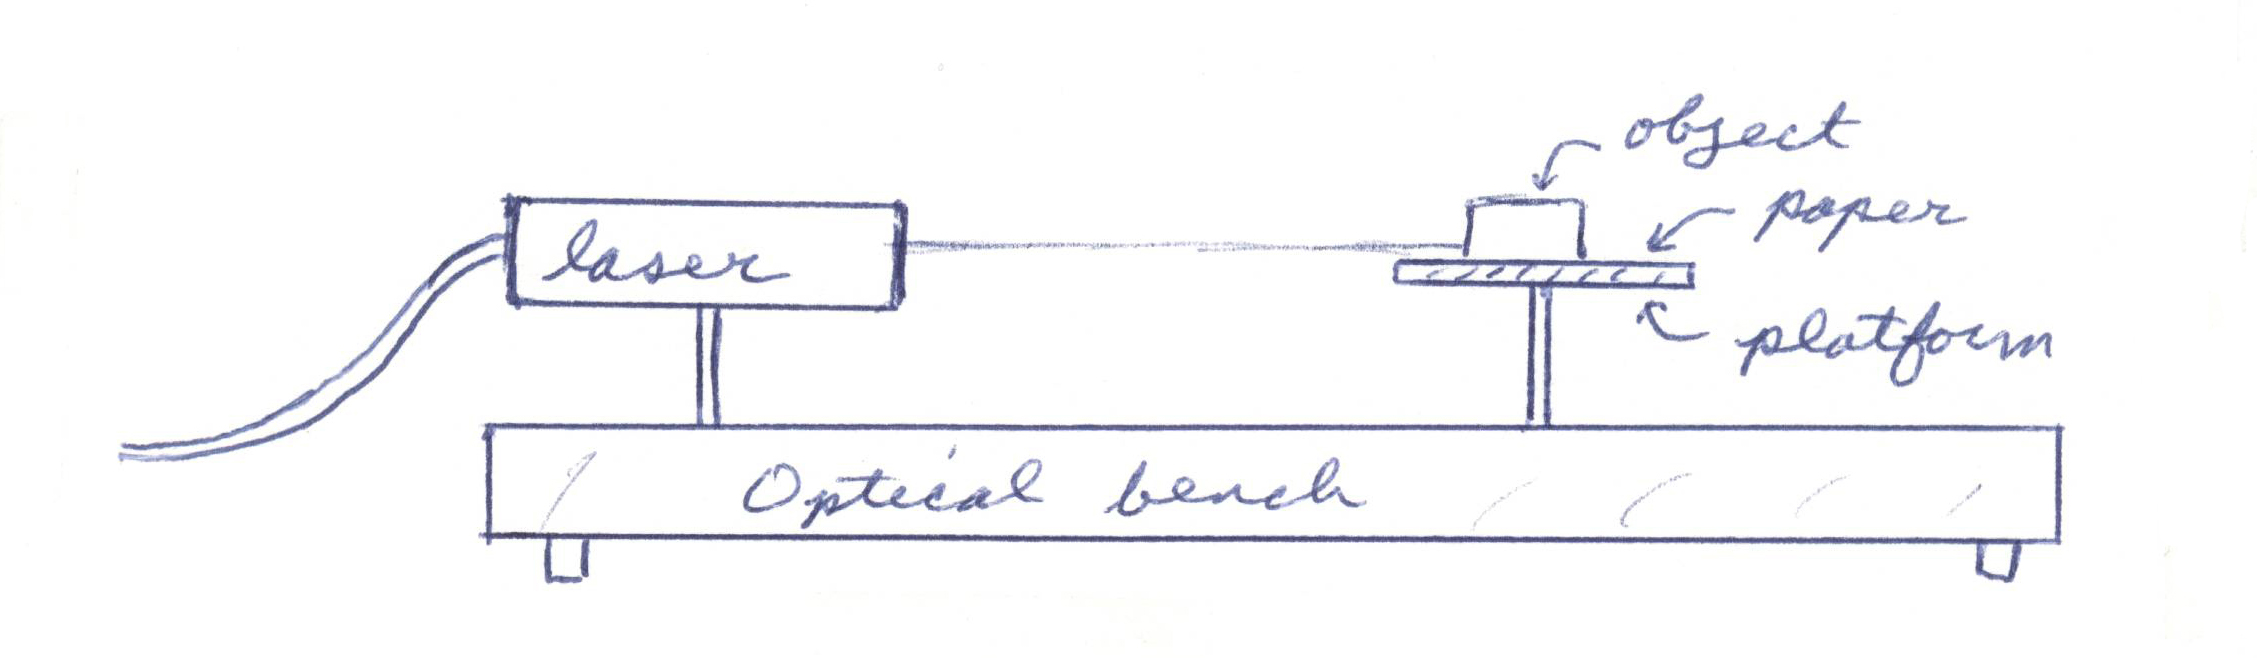
\includegraphics[scale=0.8]{5bgraf/fig_14}
%	\caption{Laser on optical bench}
%	\label{f:fig14}
%\end{figure}

\begin{center}
	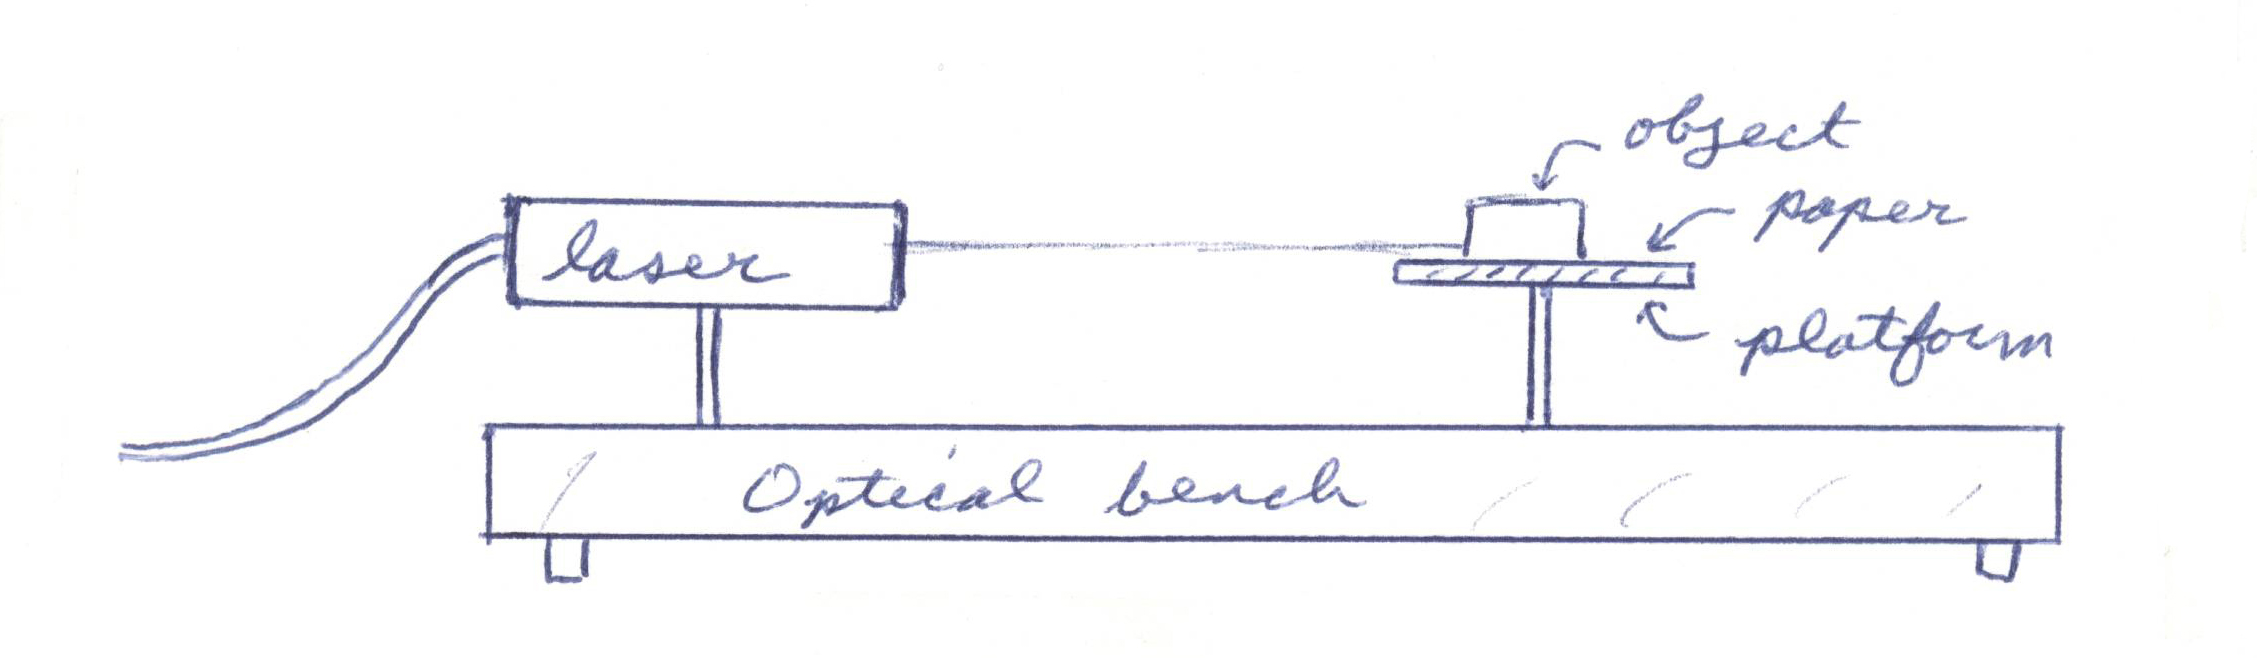
\includegraphics[scale=0.8]{5bgraf/fig_14}
	\mfcaption{Laser on optical bench}
	\label{f:fig14}
\end{center}


An optical bench is used to provide firm support for the laser and the platform on which measurements are made.  Align the laser and platform so that the beam is parallel to the surface of the platform.  Place a cork pad on the platform and a sheet of paper on top of the cork.  Pins placed judiciously can then be used to trace the path of the laser beam.

The law of reflection is particularly simple.  It is illustrated in the \reffig{f:fig15}  The angle of incidence $\theta_i$ equals the angle of reflection $\theta_r$.  The law of refraction governs the direction of light rays when their speed changes, as in passing from one medium to another.  It is illustrated in \reffig{f:fig16}.  The equation for the law of refraction is called Snell's law and is written
\begin {equation} \label{e:snell}
n_1 \ \text{sin} \ \theta_1 = n_2 \ \text{sin} \ \theta_2
\end {equation}

where $n_1$ and $n_2$ are the indices of refraction for the media involved.  

%\begin{comment}
%\begin{figure}
%	\centering
%	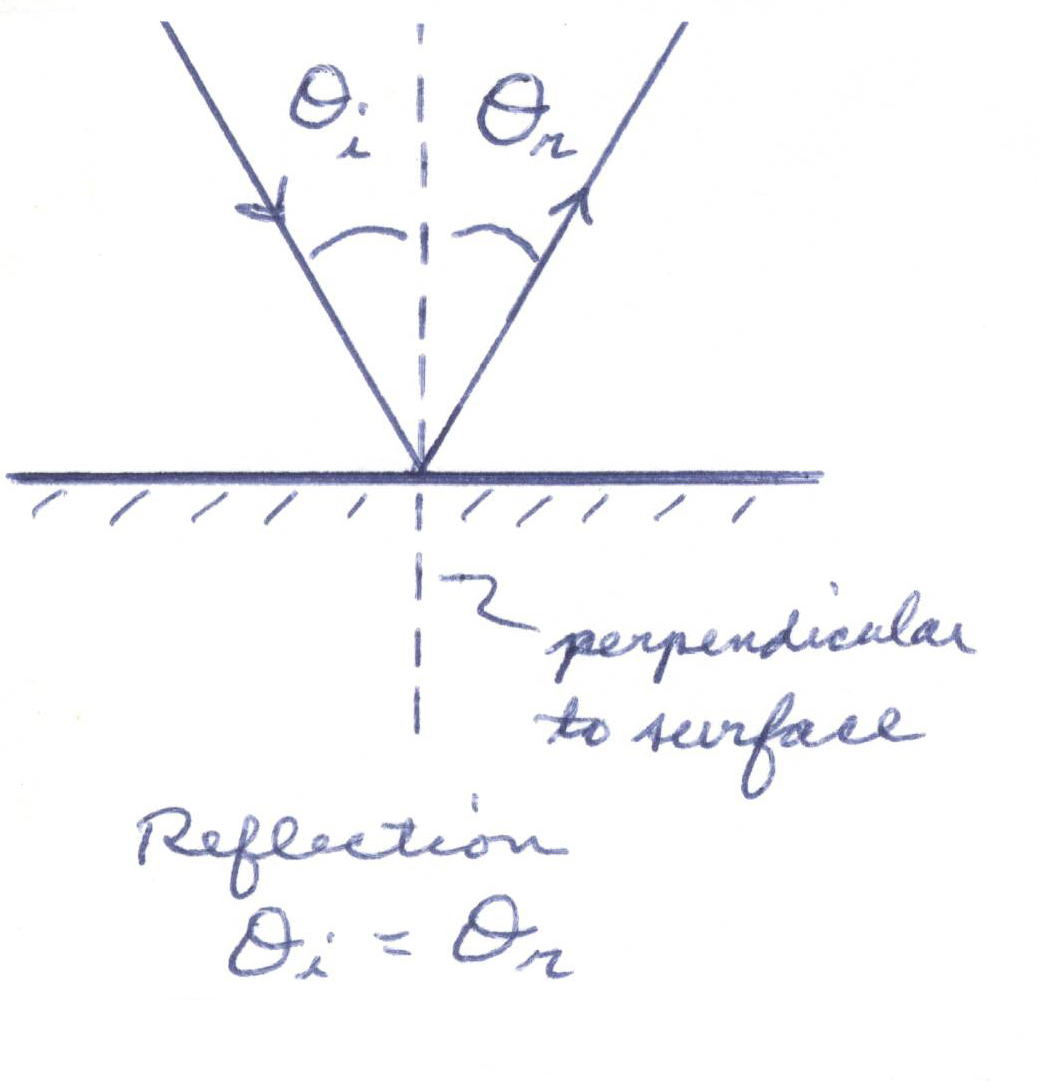
\includegraphics[scale=0.8]{5bgraf/fig_15}
%	\caption{Law of reflection}
%	\label{f:fig15}
%\end{figure}

%\begin{figure}
%	\centering
%	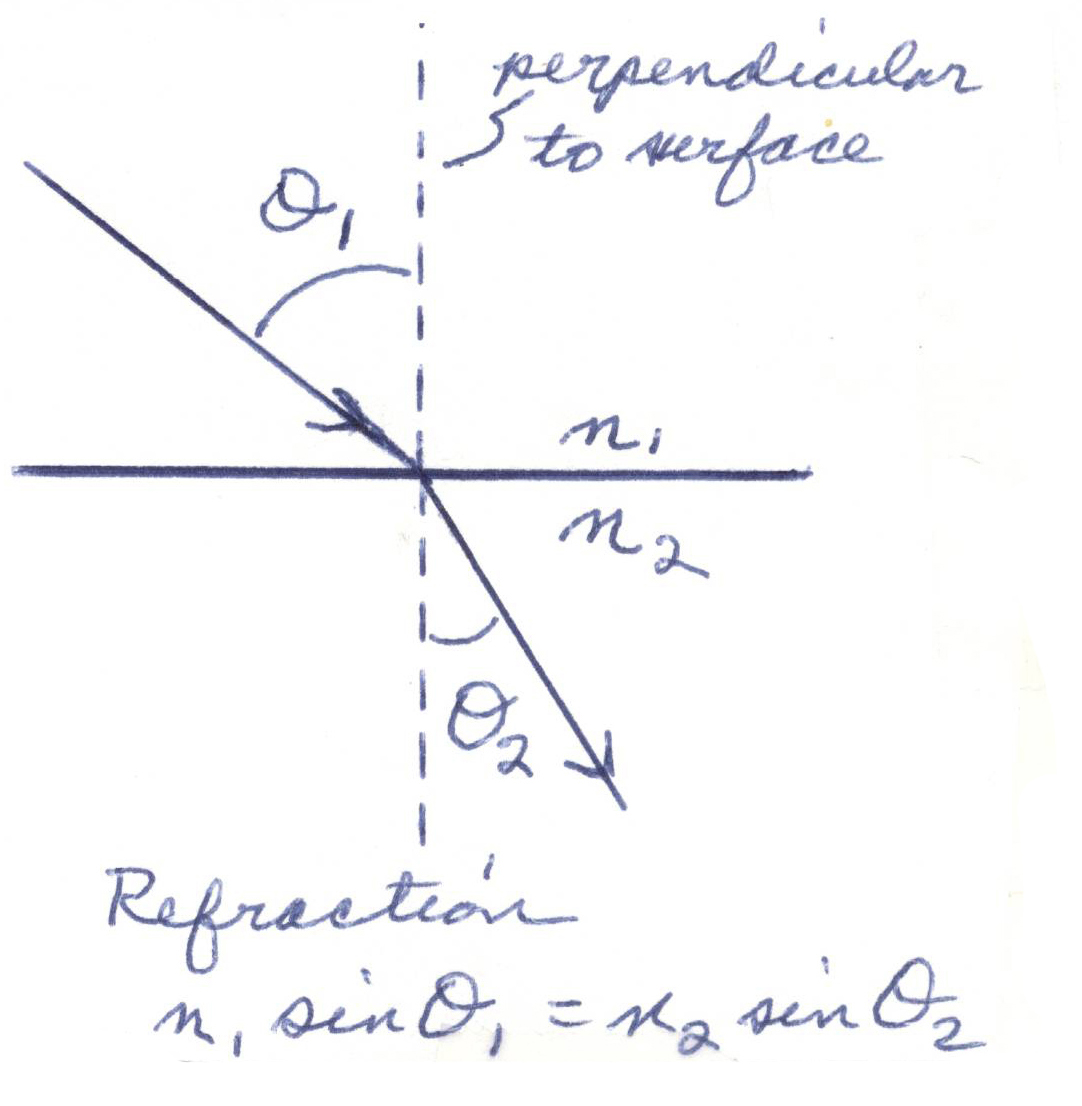
\includegraphics[scale=0.8]{5bgraf/fig_16}
%	\caption{Law of refraction}
%	\label{f:fig16}
%\end{figure}
%\end{comment}

%\begin{figure} \centering
% \subfloat[reflection]
%   {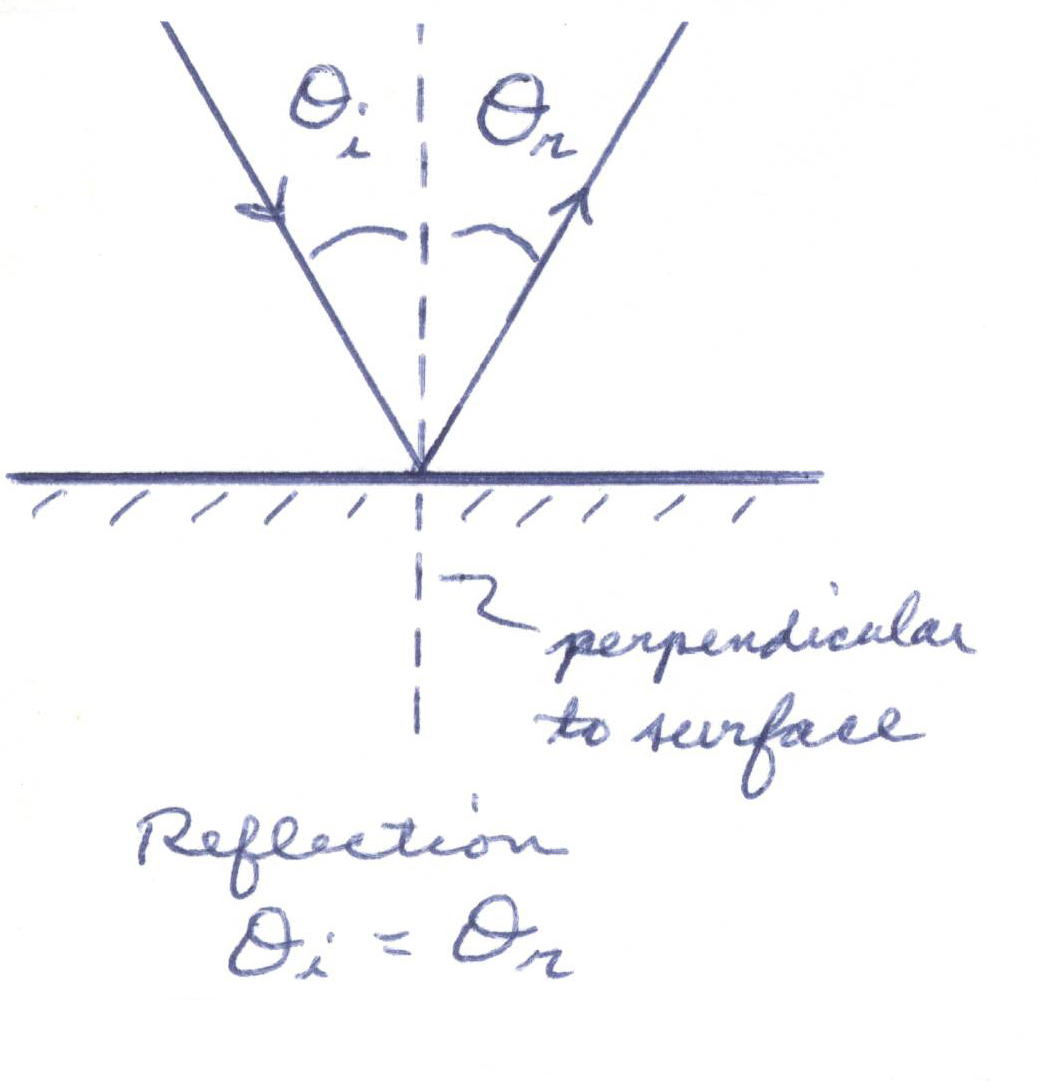
\includegraphics[scale=0.9]{5bgraf/fig_15}\label{f:fig15}}
% \qquad \qquad
% \subfloat[refraction]
%   {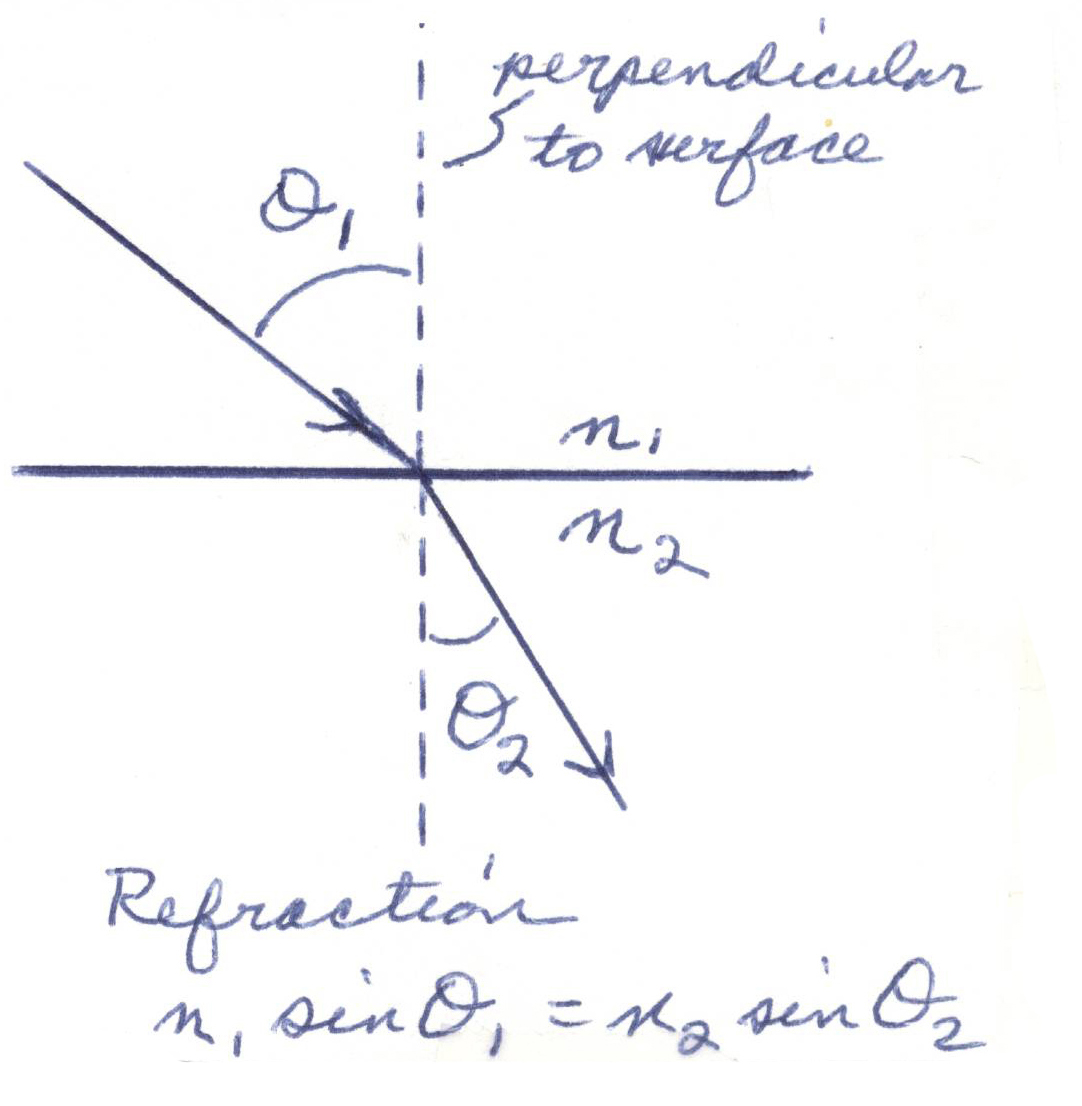
\includegraphics[scale=0.9]{5bgraf/fig_16}\label{f:fig16}}
% \caption{Laws of Reflection and Refraction}\label{f:rfract}
%\end{figure}

\begin{center}
	{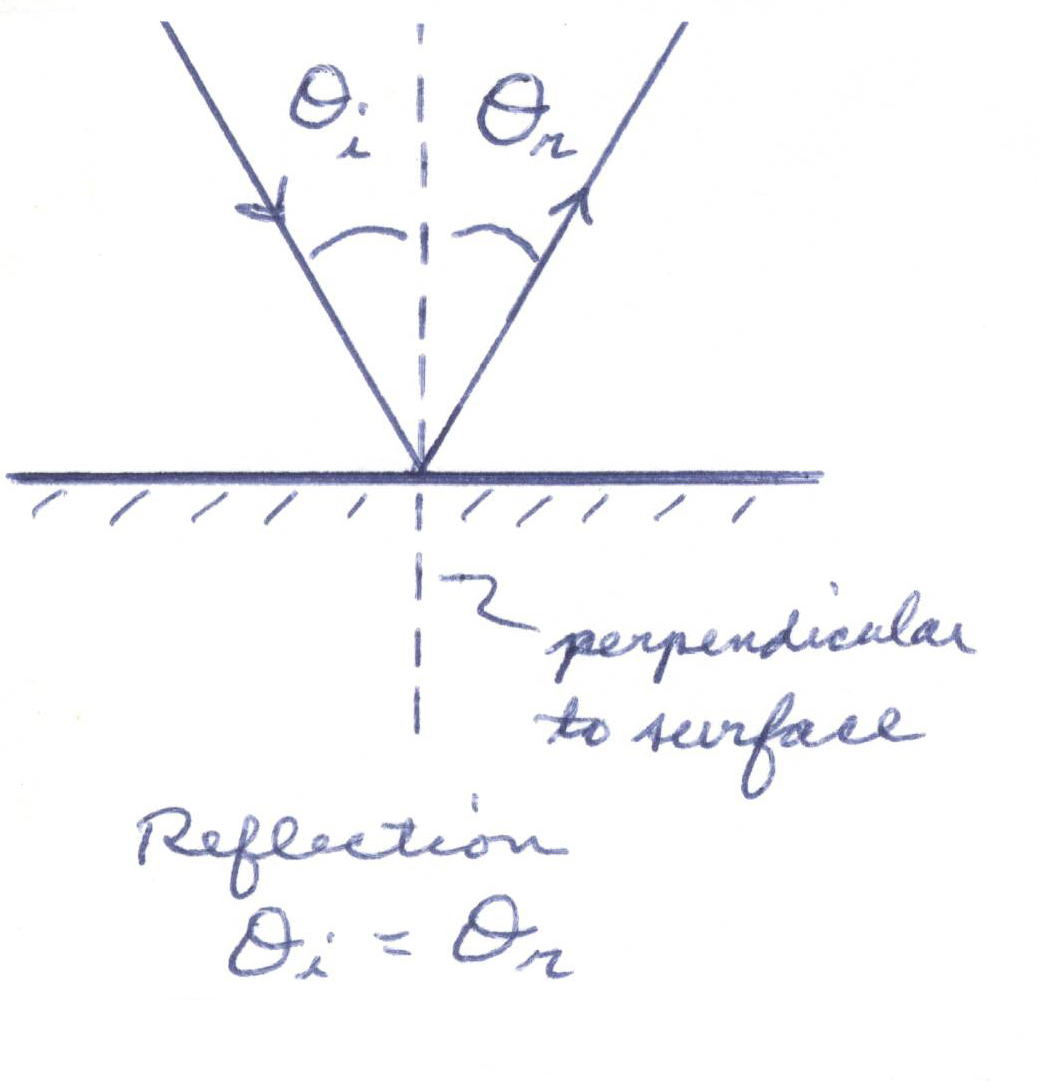
\includegraphics[scale=0.9]{5bgraf/fig_15}\label{f:fig15}}
	{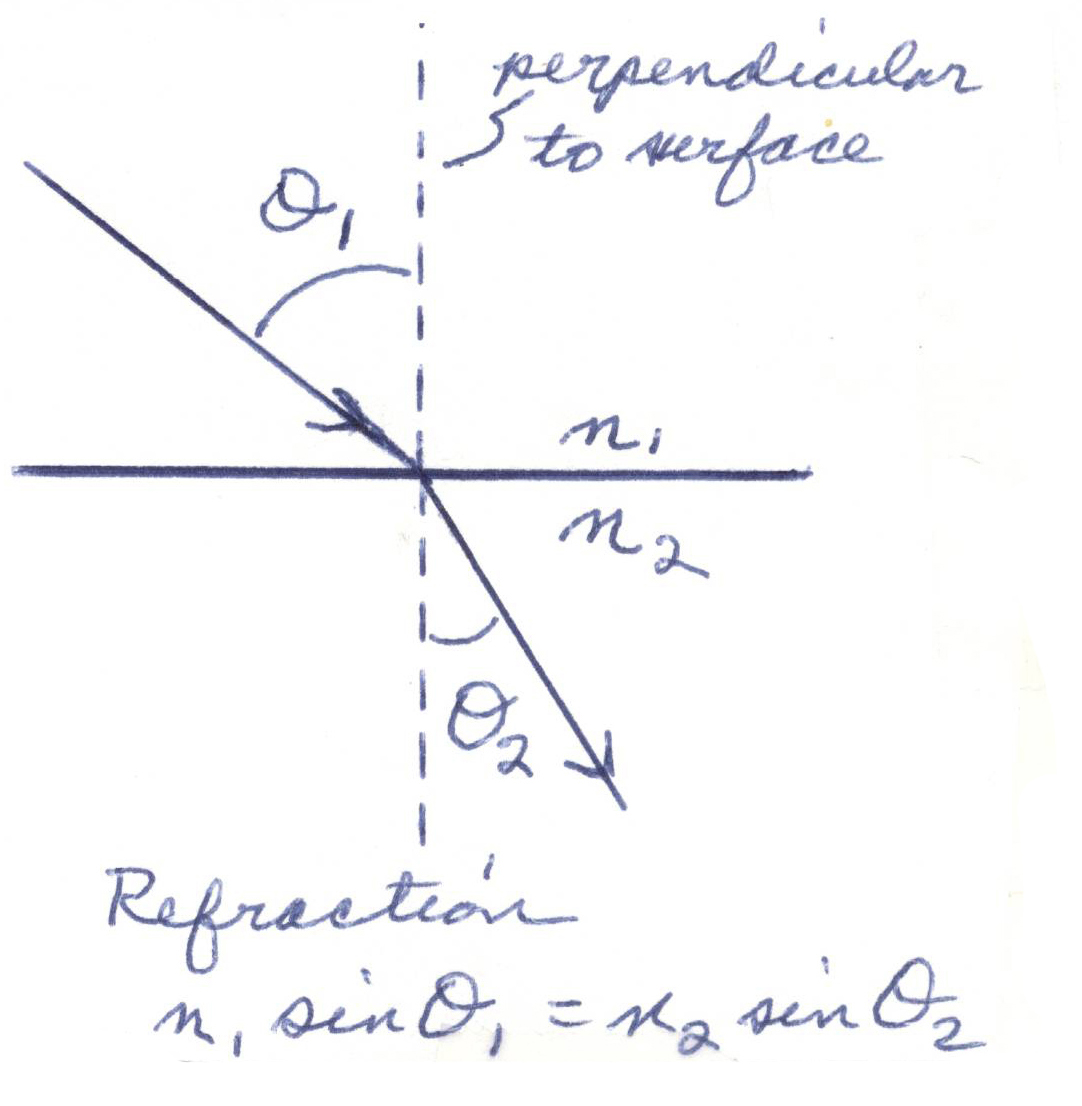
\includegraphics[scale=0.9]{5bgraf/fig_16}\label{f:fig16}}
	\mfcaption{Laws of Reflection and Refraction}\label{f:rfract}
	\label{f:fig14}
\end{center}



Note that the angles are measured relative to a line that is perpendicular to the surface at the point where the light ray meets the surface.  The perpendicular is shown as a dashed line.  You can use a protractor to draw the perpendicular.  Your instructor will guide you in both determining the perpendicular and measuring pertinent angles.

%---------------------------------------------------------------------
\section{Geometric optics: ray model}

\subsection{Activity: Reflection and Refraction}
\begin{enumerate}
% Verify the law of reflection
	\item Use the front silvered mirror to verify the law of reflection.  Make measurements for three different angles of incidence.  Discuss whether the law is verified within experimental uncertainties.

% Verify the law of refraction
	\item Partially fill the pie box with water and a small amount of powdered milk. Trace a ray of light as it enters and leaves the pie box.  
	\item Taking the index of refraction of water to be 1.33 and that of air to be 1.00, check to see if the law of refraction (Snell's law: \refeqn{e:snell}) is verified at both the entry and exit points.  As usual, the verification need only be within experimental uncertainties.
	\item Discuss your results. Also discuss why your results are not affected by the fact that the light goes through plastic as well as air and water.
\end{enumerate}
	
\subsection{Activity: Index of refraction of glass}
Trace a ray of light through a glass block and glass prism.  Using the law of refraction and your measured angles, find the index of refraction of the glass.  Take the index of refraction of air to be 1.00.  How does your value for glass compare with the values listed in your text?

\begin{equation} \label{e:critang}
	\theta_c = \sin^{-1} \left(\frac{n_2}{n_1}\right) \text{where} \ n_1 > n_2
\end{equation}
	 

\subsection{Activity: Critical angle for a glass-air surface}
Pass the ray of light through a prism.  Gradually rotate the prism so that the ray leaving the other side comes out at progressively greater angles relative to the perpendicular to the surface.  Determine at what internal angle the light no longer emerges.  The smallest such angle is the critical angle.  Compare your measured value with that calculated using equation \ref{e:critang}:

\subsection{Activity: Focal point and length}
%  Find the focal point and focal length of a concave mirror
\begin{enumerate}
	 \item 	Use the curved metal mirror to verify that the focal length of such a mirror is one half its radius of curvature.  Measure the radius of curvature $R$ of the mirror by tracing its curve with a large compass.  Then trace the paths of parallel incident rays before and after they are reflected by the mirror.  The point at which they cross after reflection is the focal point.  
	 \item Measure the distance of this point from the mirror.  This is the focal length $f$ of the mirror.  
	 \item Discuss whether $f$ is half the radius of curvature $R$, as is predicted by the law of reflection.
\end{enumerate}
	
%---------------------------------------------------------------------
\section{Conclusions}
  What general conclusions can you make concerning the laws of reflection and refraction based on your experiences in this lab?
 
% \clearpage
%\newpage
%\includegraphics*[width=\textwidth,trim=120 80 80 120,clip]{5bgraf/pslabgrid} 
\end{multicols} 
%--------------------------------------------------------------------------
\endinput
%--------------------------------------------------------------------------
